\subsection{Speckle beam design}\label{speckle_design}

\begin{figure*}
    \centering
    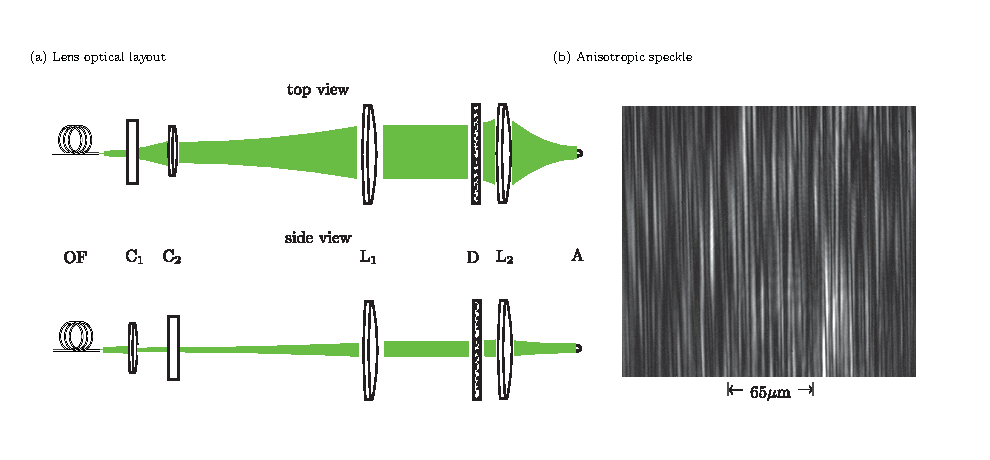
\includegraphics{Chapter6_secs/speckle_design.pdf}
    \caption{Optical design. (a). The design of optics viewed in two directions. OF denotes optical fiber. Lenses $C_1$ and $C_2$ are cylindrical lenses: $C_1$ focuses the beam in the vertical direction; and $C_2$ focuses the beam in the horizontal direction. $L_1$ is a spherical lens that collimates the beam. D is the optical diffuser that imprints random phase on the beam. $L_2$ is an aspherical lens that focuses the beam to the atoms labelled with A. (b) Experimental image of optical speckle with anisotropic correlation length.}
    \label{fig:design}
\end{figure*}

In practice, the speckle beam must satisfy two requirements.
The first is anisotropic field-field correlation length: small along $\ex$ and large along $\ey$ and $\ez$ so that high-momentum scattering occurs predominantly along $\ex$. 
The second is that the beam width along $\ex$ should uniformly illuminate the elongated atomic ensemble (with expected diameter of about $50\ \mu{\rm m}$).
To observe the effect of SOC-suppressed transport, the speckle potential must couple energy matched states across the SOC gap, shown by the dashed line in Fig.~\ref{fig:Dispersion relations}(c). 
This implies PSD of speckle potential along $\ex$ satisfies $k_c\gtrsim 4\kr$, informing the selection of beam-size and lenses.
The requirement that the correlation length along $\ey$ be large implies that at the diffuser plate, the beam be much smaller along $\ey$ than along $\ex$.

To satisfy these joint requirements, we created the speckle beam shown in Fig.~\ref{fig:design}(a), that begins with a $532{\rm nm}$ laser beam emanating from an optical fiber. 
The beam out of an optical fiber travels through the cylindrical lens $C_1$ (focusing along $\ey$) before encountering a cylindrical lens $C_2$ (focusing along $\ex$) as shown in Fig.~\ref{fig:design}(a), given more rapid divergence along $\ex$ than $\ey$.
The beam is then collimated by $L_1$, a $f = 250\ {\rm mm}$ spherical lens, giving beam width of around $25\ {\rm mm}$ along $\ex$ and less than $500\ \mu{\rm  m}$ along $\ey$ (on the same scale the diffuser plate's correlation length). 

The beam then traverses the diffuser plate (Edmund Optics part number \#47-680, with divergence angle $\theta_d = 0.5^\circ$)  and is focused by $L_2$, a $f = 30\ {\rm mm}$ lens.
Figure~\ref{fig:design}(b) shows a test image of the speckle beam at the focal plane, its intensity correlation length is less than $0.5\ {\rm \mu m}$ along $\ex$ and about $10\ \mu{\rm  m}$ along $\ey$. 
The beam widths along both directions are about $250\ \mu{\rm m}$.

